% answers.tex —— 2023 年·新高考Ⅰ卷 · 参考答案与详细解析片段
% 由 tools/generate_projects.py 依来源总账自 2023/2023_数学真题_试题.md + 2023/2023_数学真题_解析正文.md + 2023/2023_数学真题_答案要点.md 生成，勿手改（改源 MD 后重跑）


\begin{gknotice}
\textbf{解析归属}：本文档全部解析由本库编写者根据试题独立推导，\textbf{非官方标准答案}。推导过程完整给出以便核验；若与官方发布版本不一致，以官方为准。

\textbf{结构提示}：本卷为 22 题制。2024 年起改为 19 题制，故本卷宜按知识点抽题练习，不宜整套限时模拟。
\end{gknotice}

\par\medskip

\gkpart{一、单选题（每小题 5 分，共 40 分）}

\begin{answer}
\gksolhead{1}{}

\textbf{题目}：

已知集合 $M=\{-2,-1,0,1,2\}$，$N=\left\{x\mid x^{2}-x-6\ge0\right\}$，则 $M\cap N=$\mbox{（　　）}

\begin{gkopts}(4)
\task A．$\{-2,-1,0,1\}$
\task B．$\{0,1,2\}$
\task C．$\{-2\}$
\task D．$\{2\}$
\end{gkopts}

\Needspace{4\baselineskip}
\textbf{解析}

\Needspace{5\baselineskip}
先解 $N$ 的不等式，因式分解：
\nopagebreak[4]
\[x^{2}-x-6=(x-3)(x+2)\ge0\]

\Needspace{5\baselineskip}
两根为 $-2$ 与 $3$，开口向上，故解集为
\nopagebreak[4]
\[N=(-\infty,-2]\cup[3,+\infty)\]

逐个检验 $M$ 的元素：

\begin{center}
\begin{tabular}{cccccc}
\toprule
元素 & $-2$ & $-1$ & $0$ & $1$ & $2$ \\
\midrule
是否 $\le-2$ 或 $\ge3$ &  &  &  &  &  \\
\bottomrule
\end{tabular}
\end{center}

\nopagebreak[4]
\[M\cap N=\{-2\}\]

\begin{gktip}
\textbf{易错点}：不等式带等号，$x=-2$ 使 $x^2-x-6=4+2-6=0$ 满足 $\ge0$，\textbf{必须保留}。若漏掉等号会得到空集而无从选择。
\end{gktip}

\gkanswer{答案：C}

\par\medskip

\end{answer}
\begin{answer}
\gksolhead{2}{}

\textbf{题目}：

已知 $z=\dfrac{1-\mathrm i}{2+2\mathrm i}$，则 $z-\bar z=$\mbox{（　　）}

\begin{gkopts}(4)
\task A．$-\mathrm i$
\task B．$\mathrm i$
\task C．$0$
\task D．$1$
\end{gkopts}

\Needspace{4\baselineskip}
\textbf{解析}

\Needspace{5\baselineskip}
\textbf{第一步，化简 $z$。} 分母提取公因数 $2$：
\nopagebreak[4]
\[z=\frac{1-\mathrm i}{2(1+\mathrm i)}\]

\Needspace{5\baselineskip}
分子分母同乘 $(1-\mathrm i)$：
\nopagebreak[4]
\[z=\frac{(1-\mathrm i)^{2}}{2(1+\mathrm i)(1-\mathrm i)}=\frac{1-2\mathrm i+\mathrm i^{2}}{2\left(1-\mathrm i^{2}\right)}=\frac{-2\mathrm i}{4}=-\frac{\mathrm i}2\]

\textbf{第二步，求 $z-\bar z$。}

\Needspace{5\baselineskip}
设 $z=x+y\mathrm i$，则 $\bar z=x-y\mathrm i$，于是
\nopagebreak[4]
\[z-\bar z=2y\mathrm i=2\mathrm i\cdot\operatorname{Im}(z)\]

\Needspace{5\baselineskip}
此处 $z=0-\dfrac12\mathrm i$，$\operatorname{Im}(z)=-\dfrac12$：
\nopagebreak[4]
\[z-\bar z=2\mathrm i\times\left(-\frac12\right)=-\mathrm i\]

\begin{gktip}
\textbf{常用结论}（值得背下来）：$z+\bar z=2\operatorname{Re}(z)$（实数），$z-\bar z=2\mathrm i\operatorname{Im}(z)$（纯虚数或零）。有了它，本题只需求出虚部即可，不必写出完整的 $\bar z$。
\end{gktip}

\gkanswer{答案：A}

\par\medskip

\end{answer}
\begin{answer}
\gksolhead{3}{}

\textbf{题目}：

已知向量 $\boldsymbol a=(1,1)$，$\boldsymbol b=(1,-1)$。若 $(\boldsymbol a+\lambda\boldsymbol b)\perp(\boldsymbol a+\mu\boldsymbol b)$，则\mbox{（　　）}

\begin{gkopts}(4)
\task A．$\lambda+\mu=1$
\task B．$\lambda+\mu=-1$
\task C．$\lambda\mu=1$
\task D．$\lambda\mu=-1$
\end{gkopts}

\Needspace{4\baselineskip}
\textbf{解析}

\Needspace{5\baselineskip}
\textbf{方法一（坐标法）}
\nopagebreak[4]
\[\boldsymbol a+\lambda\boldsymbol b=(1+\lambda,\ 1-\lambda),\qquad \boldsymbol a+\mu\boldsymbol b=(1+\mu,\ 1-\mu)\]

\Needspace{5\baselineskip}
由垂直得数量积为零：
\nopagebreak[4]
\[(1+\lambda)(1+\mu)+(1-\lambda)(1-\mu)=0\]

\Needspace{5\baselineskip}
展开：
\nopagebreak[4]
\[\left(1+\mu+\lambda+\lambda\mu\right)+\left(1-\mu-\lambda+\lambda\mu\right)=2+2\lambda\mu=0\]

\nopagebreak[4]
\[\lambda\mu=-1\]

\textbf{方法二（整体法，更快）}

\Needspace{5\baselineskip}
先注意到本题基向量的两个特殊性质：
\nopagebreak[4]
\[\boldsymbol a\cdot\boldsymbol b=1\times1+1\times(-1)=0,\qquad |\boldsymbol a|^{2}=|\boldsymbol b|^{2}=2\]

\Needspace{5\baselineskip}
直接展开：
\nopagebreak[4]
\[(\boldsymbol a+\lambda\boldsymbol b)\cdot(\boldsymbol a+\mu\boldsymbol b)=|\boldsymbol a|^{2}+(\lambda+\mu)\underbrace{\boldsymbol a\cdot\boldsymbol b}_{=0}+\lambda\mu|\boldsymbol b|^{2}=2+2\lambda\mu=0\]

同样得 $\lambda\mu=-1$。

\begin{gktip}
\textbf{方法总结}：当基向量互相垂直且模相等时，用整体展开比代坐标更快，且不易算错。做题前先花 3 秒观察 $\boldsymbol a\cdot\boldsymbol b$ 是否为零，往往能省一半计算。
\end{gktip}

\gkanswer{答案：D（$\lambda\mu=-1$）}

\par\medskip

\end{answer}
\begin{answer}
\gksolhead{4}{}

\textbf{题目}：

设函数 $f(x)=2^{x(x-a)}$ 在区间 $(0,1)$ 单调递减，则 $a$ 的取值范围是\mbox{（　　）}

\begin{gkopts}(4)
\task A．$(-\infty,-2]$
\task B．$[-2,0)$
\task C．$(0,2]$
\task D．$[2,+\infty)$
\end{gkopts}

\Needspace{4\baselineskip}
\textbf{解析}

\textbf{第一步，识别复合结构。}

$f(x)=2^{g(x)}$，其中 $g(x)=x(x-a)=x^{2}-ax$。

\Needspace{5\baselineskip}
外层 $y=2^{u}$ 是\textbf{增函数}，由「同增异减」：
\nopagebreak[4]
\[f\ \text{\text{在}}\ (0,1)\ \text{\text{递减}}\iff g\ \text{\text{在}}\ (0,1)\ \text{\text{递减}}\]

\textbf{第二步，分析二次函数 $g$。}

\Needspace{5\baselineskip}
$g(x)=x^{2}-ax$ 开口向上，对称轴
\nopagebreak[4]
\[x=\frac a2\]

开口向上的抛物线在对称轴\textbf{左侧}单调递减，即递减区间为 $\left(-\infty,\dfrac a2\right]$。

\textbf{第三步，包含关系。}

\Needspace{5\baselineskip}
要求 $(0,1)$ 落在递减区间内：
\nopagebreak[4]
\[(0,1)\subseteq\left(-\infty,\frac a2\right]\ \Longrightarrow\ \frac a2\ge1\ \Longrightarrow\ a\ge2\]

\begin{gktip}
\textbf{方法总结}：复合函数单调性题的三步——① 拆成内外层；② 判断外层增减，用「同增异减」把结论转移到内层；③ 对内层用其自身的单调性理论（本题是二次函数的对称轴）。注意区间端点：因为 $(0,1)$ 是开区间，$\dfrac a2\ge1$ 中的等号可以取到。
\end{gktip}

\gkanswer{答案：D（$a\ge2$）}

\par\medskip

\end{answer}
\begin{answer}
\gksolhead{5}{}

\textbf{题目}：

设椭圆 $C_1:\dfrac{x^{2}}{a^{2}}+y^{2}=1\ (a>1)$，$C_2:\dfrac{x^{2}}4+y^{2}=1$ 的离心率分别为 $e_1$，$e_2$。若 $e_2=\sqrt3\,e_1$，则 $a=$\mbox{（　　）}

\begin{gkopts}(2)
\task A．$\dfrac{2\sqrt3}3$
\task B．$\sqrt2$
\task C．$\sqrt3$
\task D．$\sqrt6$
\end{gkopts}

\Needspace{4\baselineskip}
\textbf{解析}

\textbf{第一步，求 $e_2$。}

\Needspace{5\baselineskip}
$C_2$ 中 $a_2^{2}=4$，$b_2^{2}=1$，焦点在 $x$ 轴上：
\nopagebreak[4]
\[c_2=\sqrt{4-1}=\sqrt3,\qquad e_2=\frac{c_2}{a_2}=\frac{\sqrt3}2\]

\textbf{第二步，表示 $e_1$。}

\Needspace{5\baselineskip}
$C_1$ 中 $b^{2}=1$，由条件 $a>1$ 知 $a^{2}>1=b^{2}$，故\textbf{焦点也在 $x$ 轴上}：
\nopagebreak[4]
\[c_1=\sqrt{a^{2}-1},\qquad e_1=\frac{\sqrt{a^{2}-1}}a\]

\Needspace{5\baselineskip}
\textbf{第三步，代入关系式。}
\nopagebreak[4]
\[\frac{\sqrt3}2=\sqrt3\cdot\frac{\sqrt{a^{2}-1}}a\ \Longrightarrow\ \frac12=\frac{\sqrt{a^{2}-1}}a\ \Longrightarrow\ a=2\sqrt{a^{2}-1}\]

\Needspace{5\baselineskip}
两边平方：
\nopagebreak[4]
\[a^{2}=4\left(a^{2}-1\right)\ \Longrightarrow\ 3a^{2}=4\ \Longrightarrow\ a^{2}=\frac43\]

\Needspace{5\baselineskip}
因 $a>1$：
\nopagebreak[4]
\[a=\frac2{\sqrt3}=\frac{2\sqrt3}3\]

\textbf{检验}：$\dfrac{2\sqrt3}3\approx1.155>1$  符合 $a>1$。

\begin{gktip}
\textbf{注意}：条件 $a>1$ 不只是限定取值范围，更重要的是\textbf{确定了 $C_1$ 的焦点在 $x$ 轴上}。若 $0<a<1$，则长轴在 $y$ 轴上，$e_1=\dfrac{\sqrt{1-a^{2}}}1$，公式完全不同。凡见到形如 $\dfrac{x^2}{a^2}+y^2=1$ 而 $a$ 待定的椭圆，第一件事就是判断焦点位置。
\end{gktip}

\gkanswer{答案：A（$\dfrac{2\sqrt3}3$）}

\par\medskip

\end{answer}
\begin{answer}
\gksolhead{6}{}

\textbf{题目}：

过点 $(0,-2)$ 与圆 $x^{2}+y^{2}-4x-1=0$ 相切的两条直线的夹角为 $\alpha$，则 $\sin\alpha=$\mbox{（　　）}

\begin{gkopts}(2)
\task A．$1$
\task B．$\dfrac{\sqrt{15}}4$
\task C．$\dfrac{\sqrt{10}}4$
\task D．$\dfrac{\sqrt6}4$
\end{gkopts}

\Needspace{4\baselineskip}
\textbf{解析}

\Needspace{5\baselineskip}
\textbf{第一步，化圆的标准方程。}
\nopagebreak[4]
\[x^{2}-4x+y^{2}=1\ \Longrightarrow\ (x-2)^{2}+y^{2}=5\]

圆心 $C(2,0)$，半径 $r=\sqrt5$。

\textbf{第二步，算外点到圆心的距离。}

\Needspace{5\baselineskip}
设外点 $P(0,-2)$：
\nopagebreak[4]
\[d=|PC|=\sqrt{(2-0)^{2}+(0+2)^{2}}=\sqrt{4+4}=2\sqrt2\]

（$d=2\sqrt2\approx2.83>\sqrt5\approx2.24$，$P$ 在圆外，确实有两条切线。）

\textbf{第三步，用半角关系（本题核心）。}

设两条切线的夹角为 $\alpha$，由对称性，\textbf{$PC$ 是这个角的平分线}，故半角 $\theta=\dfrac\alpha2$ 满足：

\Needspace{5\baselineskip}
在切点、圆心、外点构成的直角三角形中（切线垂直于过切点的半径）：
\nopagebreak[4]
\[\sin\theta=\frac rd=\frac{\sqrt5}{2\sqrt2},\qquad \cos\theta=\frac{\sqrt{d^{2}-r^{2}}}d=\frac{\sqrt{8-5}}{2\sqrt2}=\frac{\sqrt3}{2\sqrt2}\]

\Needspace{5\baselineskip}
\textbf{第四步，二倍角。}
\nopagebreak[4]
\[\sin\alpha=\sin2\theta=2\sin\theta\cos\theta=2\times\frac{\sqrt5}{2\sqrt2}\times\frac{\sqrt3}{2\sqrt2}=\frac{2\sqrt{15}}{4\times2}=\frac{\sqrt{15}}4\]

\begin{gktip}
\textbf{常见错误}：直接把 $\dfrac rd=\dfrac{\sqrt5}{2\sqrt2}=\dfrac{\sqrt{10}}4$ 当成 $\sin\alpha$，从而错选 C——那求的是\textbf{半角}的正弦。凡涉及「两条切线夹角」，务必记住 $PC$ 平分该角，必须再做一次二倍角。
\end{gktip}

\gkanswer{答案：B（$\dfrac{\sqrt{15}}4$）}

\par\medskip

\end{answer}
\begin{answer}
\gksolhead{7}{}

\textbf{题目}：

记 $S_n$ 为数列 $\left\{a_n\right\}$ 的前 $n$ 项和，设甲：$\left\{a_n\right\}$ 为等差数列；乙：$\left\{\dfrac{S_n}n\right\}$ 为等差数列，则\mbox{（　　）}

\begin{gkopts}(2)
\task A．甲是乙的充分条件但不是必要条件
\task B．甲是乙的必要条件但不是充分条件
\task C．甲是乙的充要条件
\task D．甲既不是乙的充分条件也不是乙的必要条件
\end{gkopts}

\Needspace{4\baselineskip}
\textbf{解析}

\textbf{方向一：甲 $\Rightarrow$ 乙（充分性）}

\Needspace{5\baselineskip}
设 $\left\{a_n\right\}$ 是首项 $a_1$、公差 $d$ 的等差数列，则
\nopagebreak[4]
\[S_n=na_1+\frac{n(n-1)}2d\]

\nopagebreak[4]
\[\frac{S_n}n=a_1+\frac{n-1}2d=a_1+\frac d2(n-1)\]

这是首项 $a_1$、公差 $\dfrac d2$ 的等差数列  \textbf{充分性成立}。

\textbf{方向二：乙 $\Rightarrow$ 甲（必要性）}

\Needspace{5\baselineskip}
设 $\dfrac{S_n}n=A+(n-1)B$（首项 $A$、公差 $B$ 的等差数列），则
\nopagebreak[4]
\[S_n=n\left[A+(n-1)B\right]=Bn^{2}+(A-B)n\]

\Needspace{5\baselineskip}
\textbf{注意这是不含常数项的二次式。} 当 $n\ge2$ 时作差：
\nopagebreak[4]
\[a_n=S_n-S_{n-1}=B\left[n^{2}-(n-1)^{2}\right]+(A-B)\left[n-(n-1)\right]\]

\nopagebreak[4]
\[=B(2n-1)+(A-B)=2Bn+A-2B\]

$a_n$ 是 $n$ 的\textbf{一次函数}，故 $\left\{a_n\right\}$ 为等差数列（公差 $2B$）。

\Needspace{5\baselineskip}
\textbf{验证 $n=1$}（这一步不能省）：
\nopagebreak[4]
\[a_1=S_1=B+(A-B)=A\]

而通项公式给出 $2B\times1+A-2B=A$  一致，故公式对 $n=1$ 也成立。

\textbf{必要性成立}。

\textbf{综上，甲是乙的充要条件。}

\begin{gktip}
\Needspace{5\baselineskip}
\textbf{值得记住的等价链}：
\nopagebreak[4]
\[\left\{a_n\right\}\text{\text{等差}}\iff S_n=An^{2}+Bn\ (\text{\text{无常数项的二次式}})\iff\left\{\frac{S_n}n\right\}\text{\text{等差}}\]
这三者完全等价，在选填题中可以互相秒杀。特别注意 $S_n$ 若含常数项（如 $S_n=n^2+1$），则 $\{a_n\}$ \textbf{不是}等差数列（$a_1$ 会与通项公式脱节）。
\end{gktip}

\gkanswer{答案：C（充要条件）}

\par\medskip

\end{answer}
\begin{answer}
\gksolhead{8}{}

\textbf{题目}：

已知 $\sin(\alpha-\beta)=\dfrac13$，$\cos\alpha\sin\beta=\dfrac16$，则 $\cos(2\alpha+2\beta)=$\mbox{（　　）}

\begin{gkopts}(4)
\task A．$\dfrac79$
\task B．$\dfrac19$
\task C．$-\dfrac19$
\task D．$-\dfrac79$
\end{gkopts}

\Needspace{4\baselineskip}
\textbf{解析}

\textbf{第一步，从已知拆出两个"零件"。}

\Needspace{5\baselineskip}
由和差公式：
\nopagebreak[4]
\[\sin(\alpha-\beta)=\sin\alpha\cos\beta-\cos\alpha\sin\beta=\frac13\]

\Needspace{5\baselineskip}
已知 $\cos\alpha\sin\beta=\dfrac16$，代入得
\nopagebreak[4]
\[\sin\alpha\cos\beta=\frac13+\frac16=\frac12\]

\Needspace{5\baselineskip}
\textbf{第二步，拼出 $\sin(\alpha+\beta)$。}
\nopagebreak[4]
\[\sin(\alpha+\beta)=\sin\alpha\cos\beta+\cos\alpha\sin\beta=\frac12+\frac16=\frac23\]

\textbf{第三步，用二倍角（选对版本是关键）。}

\Needspace{5\baselineskip}
所求为 $\cos\left[2(\alpha+\beta)\right]$。二倍角余弦有三个版本：
\nopagebreak[4]
\[\cos2\theta=\cos^{2}\theta-\sin^{2}\theta=2\cos^{2}\theta-1=1-2\sin^{2}\theta\]

\Needspace{5\baselineskip}
由于我们只知道 $\sin(\alpha+\beta)$，选用\textbf{第三个版本}（只含 $\sin$），可以避开求 $\cos(\alpha+\beta)$ 时的正负号讨论：
\nopagebreak[4]
\[\cos(2\alpha+2\beta)=1-2\sin^{2}(\alpha+\beta)=1-2\times\left(\frac23\right)^{2}=1-\frac89=\frac19\]

\begin{gktip}
\textbf{方法总结}：三角求值题的核心是「\textbf{用已知的零件拼出目标}」。本题的零件是 $\sin\alpha\cos\beta$ 与 $\cos\alpha\sin\beta$——它们既能组成 $\sin(\alpha-\beta)$，也能组成 $\sin(\alpha+\beta)$。选择二倍角公式时，\textbf{优先选只涉及已知量的那个版本}，可以省掉符号讨论，这是本题最实用的技巧。
\end{gktip}

\gkanswer{答案：B（$\dfrac19$）}

\par\medskip

\end{answer}
\gkpart{二、多选题（每小题 5 分，共 20 分）}

\begin{answer}
\gksolhead{9}{}

\textbf{题目}：

有一组样本数据 $x_1,x_2,\cdots,x_6$，其中 $x_1$ 是最小值，$x_6$ 是最大值，则\mbox{（　　）}

\begin{gkopts}(1)
\task A．$x_2,x_3,x_4,x_5$ 的平均数等于 $x_1,x_2,\cdots,x_6$ 的平均数
\task B．$x_2,x_3,x_4,x_5$ 的中位数等于 $x_1,x_2,\cdots,x_6$ 的中位数
\task C．$x_2,x_3,x_4,x_5$ 的标准差不小于 $x_1,x_2,\cdots,x_6$ 的标准差
\task D．$x_2,x_3,x_4,x_5$ 的极差不大于 $x_1,x_2,\cdots,x_6$ 的极差
\end{gkopts}

\Needspace{4\baselineskip}
\textbf{解析}

\Needspace{5\baselineskip}
为讨论方便，把数据按从小到大排序（题设已保证 $x_1$ 最小、$x_6$ 最大）：
\nopagebreak[4]
\[x_1\le x_2\le x_3\le x_4\le x_5\le x_6\]

\par\medskip

\textbf{A 项（平均数）}

去掉最大值和最小值后平均数\textbf{未必不变}。

\textbf{反例}：$1,2,3,4,5,100$。
原六个数的平均数 $=\dfrac{115}6\approx19.17$；
中间四个 $2,3,4,5$ 的平均数 $=3.5$。
显然不等。

\par\medskip

\textbf{B 项（中位数）}

\begin{itemize}
\item 六个数的中位数：偶数个，取中间两个的平均，即 $\dfrac{x_3+x_4}2$。
\item 中间四个数 $x_2,x_3,x_4,x_5$ 的中位数：也是偶数个，取中间两个的平均，即 $\dfrac{x_3+x_4}2$。
\end{itemize}

两者\textbf{恒相等}  \textbf{正确}。

\begin{gktip}
这是中位数「抗极端值」特性的直接体现：去掉最大、最小各一个，中间位置不变。
\end{gktip}

\par\medskip

\textbf{C 项（标准差）}

去掉最大值和最小值后，数据变得\textbf{更集中}，标准差\textbf{不会增大}。C 断言"不小于"（即变大或不变），方向相反。

\textbf{反例}：$1,5,5,5,5,9$。
原数据平均数 $5$，方差 $=\dfrac{16+0+0+0+0+16}6=\dfrac{32}6\approx5.33$，标准差约 $2.31$；
中间四个 $5,5,5,5$ 的方差 $=0$，标准差 $=0$。
$0<2.31$，C 的断言不成立 

\par\medskip

\textbf{D 项（极差）}

\begin{itemize}
\item 中间四个数的极差 $=x_5-x_2$
\item 全部六个数的极差 $=x_6-x_1$
\end{itemize}

\Needspace{5\baselineskip}
由 $x_1\le x_2$ 与 $x_5\le x_6$：
\nopagebreak[4]
\[x_5-x_2\le x_6-x_2\le x_6-x_1\]

故极差\textbf{不大于}原极差  \textbf{正确}。

\begin{gktip}
\textbf{方法总结}：统计量的"稳健性"是本题的考点——\textbf{中位数和极差}对去掉两端极值的反应是可预测的（中位数不变、极差不增），而\textbf{平均数和标准差}会被极端值显著影响。记住这个结论，本题可以秒选。
\end{gktip}

\gkanswer{答案：BD}

\par\medskip

\end{answer}
\begin{answer}
\gksolhead{10}{}

\textbf{题目}：

噪声污染问题越来越受到重视。用声压级来度量声音的强弱，定义声压级 $L_P=20\times\lg\dfrac p{p_0}$，其中常数 $p_0\ (p_0>0)$ 是听觉下限阈值，$p$ 是实际声压。下表为不同声源的声压级：

\begin{center}
\begin{tabular}{ccc}
\toprule
声源 & 与声源的距离 $/\mathrm m$ & 声压级 $/\mathrm{dB}$ \\
\midrule
燃油汽车 & $10$ & $60\sim90$ \\
混合动力汽车 & $10$ & $50\sim60$ \\
电动汽车 & $10$ & $40$ \\
\bottomrule
\end{tabular}
\end{center}

已知在距离燃油汽车、混合动力汽车、电动汽车 $10\ \mathrm m$ 处测得实际声压分别为 $p_1$，$p_2$，$p_3$，则\mbox{（　　）}

\begin{gkopts}(4)
\task A．$p_1\ge p_2$
\task B．$p_2>10p_3$
\task C．$p_3=100p_0$
\task D．$p_1\le100p_2$
\end{gkopts}

\Needspace{4\baselineskip}
\textbf{解析}

\textbf{第一步，把声压级反解成声压比。}

\Needspace{5\baselineskip}
由 $L_P=20\lg\dfrac p{p_0}$：
\nopagebreak[4]
\[\lg\frac p{p_0}=\frac{L_P}{20}\ \Longrightarrow\ \frac p{p_0}=10^{L_P/20}\]

\textbf{第二步，逐个算出三者的范围。}

\begin{center}
\begin{tabular}{lcl}
\toprule
声源 & $L_P$ 范围 & $\dfrac p{p_0}$ 范围 \\
\midrule
燃油车 & $[60,90]$ & $\left[10^{3},\ 10^{4.5}\right]$ \\
混动车 & $[50,60]$ & $\left[10^{2.5},\ 10^{3}\right]$ \\
电动车 & $40$ & $10^{2}=100$ \\
\bottomrule
\end{tabular}
\end{center}

（$10^{2.5}=10^2\sqrt{10}\approx316$，$10^{4.5}\approx31623$。）

\par\medskip

\Needspace{5\baselineskip}
\textbf{A 项：$p_1\ge p_2$ }

\nopagebreak[4]
\[p_1\ge10^{3}p_0\quad\text{\text{且}}\quad p_2\le10^{3}p_0\]

故必有 $p_1\ge p_2$  \textbf{正确}（两个区间恰好在 $10^3$ 处相接）。

\par\medskip

\Needspace{5\baselineskip}
\textbf{B 项：$p_2>10p_3$ }

\nopagebreak[4]
\[10p_3=10\times100p_0=1000p_0=10^{3}p_0\]

而 $p_2$ 的\textbf{下界}为 $10^{2.5}p_0\approx316p_0<10^{3}p_0$。

取 $L_2=50$（混动车最安静的情形），则 $p_2\approx316p_0<10p_3$，不满足  \textbf{错误}。

\par\medskip

\Needspace{5\baselineskip}
\textbf{C 项：$p_3=100p_0$ }

\nopagebreak[4]
\[\frac{p_3}{p_0}=10^{40/20}=10^{2}=100\]

 \textbf{正确}（这是唯一确定值，因电动车声压级恰为 $40$）。

\par\medskip

\Needspace{5\baselineskip}
\textbf{D 项：$p_1\le100p_2$ }

\nopagebreak[4]
\[p_1\le10^{4.5}p_0\quad\text{（\text{上界}）}\]
\nopagebreak[4]
\[100p_2\ge100\times10^{2.5}p_0=10^{2}\times10^{2.5}p_0=10^{4.5}p_0\quad\text{（\text{下界}）}\]

\Needspace{5\baselineskip}
故恒有
\nopagebreak[4]
\[p_1\le10^{4.5}p_0\le100p_2\]

 \textbf{正确}（两个界恰好相等，这是命题人精心设计的"卡边"）。

\begin{gktip}
\textbf{方法总结}：对数型应用题一律先\textbf{反解成指数形式}，把所有量化成 $p_0$ 的倍数后再比较。本题四个选项都是在比较区间的\textbf{端点}，所以只需算出每个量的上下界，逐项对照即可，不必考虑中间取值。
\end{gktip}

\gkanswer{答案：ACD}

\par\medskip

\end{answer}
\begin{answer}
\gksolhead{11}{}

\textbf{题目}：

已知函数 $f(x)$ 的定义域为 $\mathbf R$，$f(xy)=y^{2}f(x)+x^{2}f(y)$，则\mbox{（　　）}

\begin{gkopts}(2)
\task A．$f(0)=0$
\task B．$f(1)=0$
\task C．$f(x)$ 是偶函数
\task D．$x=0$ 为 $f(x)$ 的极小值点
\end{gkopts}

\Needspace{4\baselineskip}
\textbf{解析}

\textbf{抽象函数方程的通法：代入特殊值。}

\par\medskip

\Needspace{5\baselineskip}
\textbf{A 项}：令 $x=y=0$：
\nopagebreak[4]
\[f(0)=0^{2}\cdot f(0)+0^{2}\cdot f(0)=0\]
 \textbf{正确}。

\par\medskip

\Needspace{5\baselineskip}
\textbf{B 项}：令 $x=y=1$：
\nopagebreak[4]
\[f(1)=1^{2}\cdot f(1)+1^{2}\cdot f(1)=2f(1)\ \Longrightarrow\ f(1)=0\]
 \textbf{正确}。

\par\medskip

\textbf{C 项}（判断奇偶性）：

\Needspace{5\baselineskip}
\textbf{先求 $f(-1)$}。令 $x=y=-1$：
\nopagebreak[4]
\[f(1)=(-1)^{2}f(-1)+(-1)^{2}f(-1)=2f(-1)\]

\Needspace{5\baselineskip}
由 B 项 $f(1)=0$，得
\nopagebreak[4]
\[f(-1)=0\]

\Needspace{5\baselineskip}
\textbf{再令 $y=-1$}（$x$ 任意）：
\nopagebreak[4]
\[f(-x)=(-1)^{2}f(x)+x^{2}f(-1)=f(x)+x^{2}\times0=f(x)\]

故 $f(-x)=f(x)$ 对一切 $x\in\mathbf R$ 成立，$f$ 是\textbf{偶函数}  \textbf{正确}。

\par\medskip

\textbf{D 项}（判断 $x=0$ 是否为极小值点）

抽象函数方程通常\textbf{不能唯一确定} $f$，因此判断"是否一定成立"要看能否找到反例。

\Needspace{5\baselineskip}
\textbf{构造反例}：取
\nopagebreak[4]
\[f(x)=\begin{cases}x^{2}\ln|x|,&x\ne0\\ 0,&x=0\end{cases}\]

\Needspace{5\baselineskip}
\textbf{验证它满足方程}（$x,y\ne0$ 时）：
\nopagebreak[4]
\[f(xy)=(xy)^{2}\ln|xy|=x^{2}y^{2}\left(\ln|x|+\ln|y|\right)=y^{2}\underbrace{\left(x^{2}\ln|x|\right)}_{f(x)}+x^{2}\underbrace{\left(y^{2}\ln|y|\right)}_{f(y)}\quad\checkmark\]

（当 $x$ 或 $y$ 为 $0$ 时两边均为 $0$，也成立。）

\Needspace{5\baselineskip}
\textbf{考察 $x=0$ 附近}：当 $0<|x|<1$ 时 $\ln|x|<0$，故
\nopagebreak[4]
\[f(x)=x^{2}\ln|x|<0=f(0)\]

即在 $x=0$ 的去心邻域内 $f(x)<f(0)$，说明 $x=0$ 是\textbf{极大值点}而非极小值点  \textbf{错误}。

\begin{gktip}
\textbf{方法总结}：抽象函数方程题分两类——
① \textbf{可以推出的性质}（A、B、C）：靠\textbf{代特殊值}（$0,1,-1$，或令 $y=-1$、$y=\dfrac1x$ 等）逐步挖掘；
② \textbf{不一定成立的性质}（D）：必须\textbf{构造反例}。构造思路是找一个满足方程的具体函数，本题的 $x^2\ln|x|$ 来自方程的"乘法变加法"结构——$f(xy)$ 中出现 $\ln|xy|=\ln|x|+\ln|y|$ 正好对应。
\end{gktip}

\gkanswer{答案：ABC}

\par\medskip

\end{answer}
\begin{answer}
\gksolhead{12}{}

\textbf{题目}：

下列物体中，能被整体放入棱长为 $1$（单位：$\mathrm m$）的正方体容器（容器壁厚度忽略不计）内的有\mbox{（　　）}

\begin{gkopts}(1)
\task A．直径为 $0.99\ \mathrm m$ 的球体
\task B．所有棱长均为 $1.4\ \mathrm m$ 的四面体
\task C．底面直径为 $0.01\ \mathrm m$，高为 $1.8\ \mathrm m$ 的圆柱体
\task D．底面直径为 $1.2\ \mathrm m$，高为 $0.01\ \mathrm m$ 的圆柱体
\end{gkopts}

\Needspace{4\baselineskip}
\textbf{解析}

\par\medskip

\textbf{A 项：直径 $0.99\ \mathrm m$ 的球 }

正方体的内切球直径为 $1\ \mathrm m$，而 $0.99<1$，直接正放即可 

\par\medskip

\textbf{B 项：棱长 $1.4\ \mathrm m$ 的正四面体 }

\Needspace{5\baselineskip}
\textbf{关键结论}：在棱长为 $1$ 的正方体中，取\textbf{四个两两不相邻的顶点}（即一条体对角线两端以外的交错顶点），它们构成一个正四面体，其棱长就是正方体的\textbf{面对角线}：
\nopagebreak[4]
\[\sqrt2\approx1.41421\]

因 $1.4<1.41421$，该正四面体可以放入 

\begin{gktip}
这个"正方体内嵌正四面体"是立体几何的经典模型，四个顶点可取 $A_1BC_1D$ 之类的组合。
\end{gktip}

\par\medskip

\textbf{C 项：底面直径 $0.01\ \mathrm m$、高 $1.8\ \mathrm m$ 的圆柱 }

这是一根很细但很长的杆。判断依据是：

\Needspace{5\baselineskip}
\textbf{正方体内所能容纳的最长线段是体对角线}，长度为
\nopagebreak[4]
\[\sqrt{1^{2}+1^{2}+1^{2}}=\sqrt3\approx1.732\]

而圆柱的高（即杆的长度）为 $1.8>1.732$，无论怎么摆放都放不进去 

\par\medskip

\textbf{D 项：底面直径 $1.2\ \mathrm m$、高 $0.01\ \mathrm m$ 的圆柱 }

这是一个很薄的圆盘，问题归结为：\textbf{棱长 $1$ 的正方体内能否放下直径 $1.2$ 的圆？}

\textbf{关键构造}：作过正方体中心且\textbf{垂直于体对角线}的截面，得到一个\textbf{正六边形}。

\Needspace{5\baselineskip}
该正六边形的边长为
\nopagebreak[4]
\[\frac{\sqrt2}2\]

（它的六个顶点是正方体六条棱的中点。）

\Needspace{5\baselineskip}
正六边形的\textbf{内切圆半径}为边长的 $\dfrac{\sqrt3}2$ 倍：
\nopagebreak[4]
\[R=\frac{\sqrt3}2\times\frac{\sqrt2}2=\frac{\sqrt6}4\approx0.6124\]

\Needspace{5\baselineskip}
内切圆直径
\nopagebreak[4]
\[2R=\frac{\sqrt6}2\approx1.2247>1.2\quad\checkmark\]

所以直径 $1.2$ 的圆盘可以沿这个"斜截面"方向放入；圆盘厚度仅 $0.01$，而余量约 $0.0247$，足够容纳  \textbf{正确}

\begin{gktip}
\textbf{方法总结}：这是一道考"正方体的三个极限尺寸"的题，值得把这三个数记熟：
\begin{itemize}
\item \textbf{最长线段}（体对角线）：$\sqrt3\approx1.732$ → 判断细长杆
\item \textbf{最大内嵌正四面体棱长}（面对角线）：$\sqrt2\approx1.414$ → 判断四面体
\item \textbf{最大内嵌圆直径}（正六边形截面的内切圆）：$\dfrac{\sqrt6}2\approx1.225$ → 判断薄圆盘
\end{itemize}

三个数由大到小依次是 $1.732>1.414>1.225>1$，对应三类不同形状的物体。
\end{gktip}

\gkanswer{答案：ABD}

\par\medskip

\end{answer}
\gkpart{三、填空题（每小题 5 分，共 20 分）}

\begin{answer}
\gksolhead{13}{}

\textbf{题目}：

某学校开设了 $4$ 门体育类选修课和 $4$ 门艺术类选修课，学生需从这 $8$ 门课中选修 $2$ 门或 $3$ 门，并且每类选修课至少选修 $1$ 门，则不同的选课方案共有 \gkblank{} 种（用数字作答）。

\Needspace{4\baselineskip}
\textbf{解析}

\textbf{按选课总数分类。}

\textbf{情况一：选 $2$ 门。}

\Needspace{5\baselineskip}
要求每类至少 $1$ 门，$2$ 门只能是"体育 $1$ 门 + 艺术 $1$ 门"：
\nopagebreak[4]
\[C_4^{1}\times C_4^{1}=4\times4=16\]

\textbf{情况二：选 $3$ 门。}

每类至少 $1$ 门，故只有两种搭配：

\begin{itemize}
\item 体育 $2$ 门 + 艺术 $1$ 门：$C_4^{2}\times C_4^{1}=6\times4=24$
\item 体育 $1$ 门 + 艺术 $2$ 门：$C_4^{1}\times C_4^{2}=4\times6=24$
\end{itemize}

小计：$24+24=48$

\Needspace{5\baselineskip}
\textbf{合计}（分类加法原理）：
\nopagebreak[4]
\[16+48=64\]

\begin{gktip}
\textbf{易错点}：① 漏掉"选 3 门"中的某一种搭配；② 用"总数减去不合要求"的补集法时容易算错（$C_8^2+C_8^3-\text{\text{全同类}}=28+56-(C_4^2\times2)-(C_4^3\times2)=84-12-8=64$，结果一致，但步骤更多）。\textbf{直接分类更稳。}
\end{gktip}

\gkanswer{答案：$64$}

\par\medskip

\end{answer}
\begin{answer}
\gksolhead{14}{}

\textbf{题目}：

在正四棱台 $ABCD\text{-}A_1B_1C_1D_1$ 中，$AB=2$，$A_1B_1=1$，$AA_1=\sqrt2$，则该棱台的体积为 \gkblank{}．

\Needspace{4\baselineskip}
\textbf{解析}

\textbf{第一步，求棱台的高（关键步骤）。}

正四棱台上下底面都是正方形，中心连线垂直于两底面。

\begin{itemize}
\item 下底正方形边长 $2$，中心到顶点距离（半对角线）$=\dfrac{2\sqrt2}2=\sqrt2$
\item 上底正方形边长 $1$，中心到顶点距离 $=\dfrac{\sqrt2}2$
\end{itemize}

\Needspace{5\baselineskip}
把侧棱 $AA_1$ 投影到底面上，投影长度为两个半对角线之差：
\nopagebreak[4]
\[\sqrt2-\frac{\sqrt2}2=\frac{\sqrt2}2\]

\Needspace{5\baselineskip}
由勾股定理求高：
\nopagebreak[4]
\[h=\sqrt{AA_1^{2}-\left(\frac{\sqrt2}2\right)^{2}}=\sqrt{2-\frac12}=\sqrt{\frac32}=\frac{\sqrt6}2\]

\Needspace{5\baselineskip}
\textbf{第二步，代入棱台体积公式。}
\nopagebreak[4]
\[V=\frac h3\left(S_{\text{\text{上}}}+S_{\text{\text{下}}}+\sqrt{S_{\text{\text{上}}}S_{\text{\text{下}}}}\right)\]

\Needspace{5\baselineskip}
其中 $S_{\text{\text{上}}}=1^{2}=1$，$S_{\text{\text{下}}}=2^{2}=4$，$\sqrt{S_{\text{\text{上}}}S_{\text{\text{下}}}}=\sqrt4=2$：
\nopagebreak[4]
\[V=\frac{\sqrt6/2}3\times(1+4+2)=\frac{\sqrt6}6\times7=\frac{7\sqrt6}6\]

\begin{gktip}
\textbf{易错点}：求高时用"边长之差"而非"半对角线之差"。正确的做法是把侧棱投影到底面，投影的起点是下底顶点、终点是上底顶点在下底的投影，这段长度等于\textbf{两个半对角线的差}（因为上下底中心在同一竖直线上）。
\end{gktip}

\gkanswer{答案：$\dfrac{7\sqrt6}6$}

\par\medskip

\end{answer}
\begin{answer}
\gksolhead{15}{}

\textbf{题目}：

已知函数 $f(x)=\cos\omega x-1\ (\omega>0)$ 在区间 $[0,2\pi]$ 有且仅有 $3$ 个零点，则 $\omega$ 的取值范围是 \gkblank{}．

\Needspace{4\baselineskip}
\textbf{解析}

\Needspace{5\baselineskip}
\textbf{第一步，解出零点。}
\nopagebreak[4]
\[f(x)=0\iff\cos\omega x=1\iff\omega x=2k\pi\ (k\in\mathbb Z)\iff x=\frac{2k\pi}\omega\]

\Needspace{5\baselineskip}
因 $\omega>0$ 且 $x\in[0,2\pi]$，零点依次为
\nopagebreak[4]
\[x_0=0,\quad x_1=\frac{2\pi}\omega,\quad x_2=\frac{4\pi}\omega,\quad x_3=\frac{6\pi}\omega,\ \cdots\]

\textbf{注意 $x=0$ 也是零点}（$\cos0=1$），这一点最容易漏。

\textbf{第二步，"恰有 3 个"的条件。}

\Needspace{5\baselineskip}
要求 $x_0,x_1,x_2$ 落在 $[0,2\pi]$ 内，而 $x_3$ 落在区间外：
\nopagebreak[4]
\[\begin{cases}\dfrac{4\pi}\omega\le2\pi\\[3mm] \dfrac{6\pi}\omega>2\pi\end{cases}\]

\Needspace{5\baselineskip}
\textbf{解第一式}（$\omega>0$，可交叉相乘）：
\nopagebreak[4]
\[4\pi\le2\pi\omega\ \Longrightarrow\ \omega\ge2\]

\Needspace{5\baselineskip}
\textbf{解第二式}：
\nopagebreak[4]
\[6\pi>2\pi\omega\ \Longrightarrow\ \omega<3\]

\Needspace{5\baselineskip}
\textbf{取交集}：
\nopagebreak[4]
\[2\le\omega<3\]

\begin{gktip}
\textbf{端点检验}（务必做）：
\begin{itemize}
\item $\omega=2$：零点为 $0,\pi,2\pi$，恰好 3 个，且 $2\pi$ 在闭区间内  故左端点\textbf{取到}。
\item $\omega=3$：零点为 $0,\dfrac{2\pi}3,\dfrac{4\pi}3,2\pi$，共 4 个  故右端点\textbf{取不到}。
\end{itemize}

这类题的分数几乎全在端点的开闭上，代入验算是最可靠的确认方式。
\end{gktip}

\gkanswer{答案：$[2,3)$}

\par\medskip

\end{answer}
\begin{answer}
\gksolhead{16}{}

\textbf{题目}：

已知双曲线 $C:\dfrac{x^{2}}{a^{2}}-\dfrac{y^{2}}{b^{2}}=1\ (a>0,\ b>0)$ 的左、右焦点分别为 $F_1$，$F_2$。点 $A$ 在 $C$ 上，点 $B$ 在 $y$ 轴上，$\overrightarrow{F_1A}\perp\overrightarrow{F_1B}$，$\overrightarrow{F_2A}=-\dfrac23\overrightarrow{F_2B}$，则 $C$ 的离心率为 \gkblank{}．

\Needspace{4\baselineskip}
\textbf{解析}

\textbf{第一步，用向量关系定出 $A$ 的坐标。}

\Needspace{5\baselineskip}
设 $F_1(-c,0)$，$F_2(c,0)$，$B\left(0,b_0\right)$（$B$ 在 $y$ 轴上）。

\nopagebreak[4]
\[\overrightarrow{F_2B}=(0-c,\ b_0-0)=\left(-c,\ b_0\right)\]

\Needspace{5\baselineskip}
由 $\overrightarrow{F_2A}=-\dfrac23\overrightarrow{F_2B}$：
\nopagebreak[4]
\[\overrightarrow{F_2A}=\left(\frac{2c}3,\ -\frac{2b_0}3\right)\]

\nopagebreak[4]
\[A=F_2+\overrightarrow{F_2A}=\left(c+\frac{2c}3,\ -\frac{2b_0}3\right)=\left(\frac{5c}3,\ -\frac{2b_0}3\right)\]

\Needspace{5\baselineskip}
\textbf{第二步，用垂直条件消去 $b_0$。}

\nopagebreak[4]
\[\overrightarrow{F_1A}=A-F_1=\left(\frac{5c}3+c,\ -\frac{2b_0}3\right)=\left(\frac{8c}3,\ -\frac{2b_0}3\right)\]
\nopagebreak[4]
\[\overrightarrow{F_1B}=\left(0+c,\ b_0\right)=\left(c,\ b_0\right)\]

\Needspace{5\baselineskip}
由 $\overrightarrow{F_1A}\cdot\overrightarrow{F_1B}=0$：
\nopagebreak[4]
\[\frac{8c}3\cdot c+\left(-\frac{2b_0}3\right)b_0=0\ \Longrightarrow\ \frac{8c^{2}}3=\frac{2b_0^{2}}3\ \Longrightarrow\ b_0^{2}=4c^{2}\]

\Needspace{5\baselineskip}
取 $b_0=2c$（取 $-2c$ 时由对称性结果相同），于是
\nopagebreak[4]
\[A\left(\frac{5c}3,\ -\frac{4c}3\right)\]

\Needspace{5\baselineskip}
\textbf{第三步，代入双曲线方程。}
\nopagebreak[4]
\[\frac{\left(\dfrac{5c}3\right)^{2}}{a^{2}}-\frac{\left(\dfrac{4c}3\right)^{2}}{b^{2}}=1\ \Longrightarrow\ \frac{25c^{2}}{9a^{2}}-\frac{16c^{2}}{9b^{2}}=1\]

\Needspace{5\baselineskip}
用 $b^{2}=c^{2}-a^{2}$，并令 $e=\dfrac ca$（即 $c^{2}=e^{2}a^{2}$）：
\nopagebreak[4]
\[\frac{25e^{2}}9-\frac{16e^{2}a^{2}}{9\left(e^{2}a^{2}-a^{2}\right)}=1\ \Longrightarrow\ \frac{25e^{2}}9-\frac{16e^{2}}{9\left(e^{2}-1\right)}=1\]

\Needspace{5\baselineskip}
两边乘 $9\left(e^{2}-1\right)$：
\nopagebreak[4]
\[25e^{2}\left(e^{2}-1\right)-16e^{2}=9\left(e^{2}-1\right)\]
\nopagebreak[4]
\[25e^{4}-25e^{2}-16e^{2}=9e^{2}-9\]
\nopagebreak[4]
\[25e^{4}-50e^{2}+9=0\]

\Needspace{5\baselineskip}
\textbf{第四步，解关于 $e^{2}$ 的二次方程。}
\nopagebreak[4]
\[e^{2}=\frac{50\pm\sqrt{2500-900}}{50}=\frac{50\pm40}{50}\]

\nopagebreak[4]
\[e^{2}=\frac95\quad\text{\text{或}}\quad e^{2}=\frac15\]

\Needspace{5\baselineskip}
双曲线要求 $e>1$，故舍去 $e^{2}=\dfrac15$：
\nopagebreak[4]
\[e=\sqrt{\frac95}=\frac3{\sqrt5}=\frac{3\sqrt5}5\]

\begin{gktip}
\textbf{检验}：$\dfrac{3\sqrt5}5=\dfrac35\sqrt5\approx1.342>1$  符合双曲线离心率的要求。

\textbf{方法总结}：解析几何中"多个向量条件求离心率"的通法是——用向量关系把动点坐标\textbf{全部化成 $c$ 的倍数}，代入曲线方程后除以 $a^2$，自然出现关于 $e$ 的方程。本题中 $b_0$ 是一个"过渡量"，它在第二步被消掉，这是设参数时值得预判的。
\end{gktip}

\gkanswer{答案：$\dfrac{3\sqrt5}5$}

\par\medskip

\end{answer}
\gkpart{四、解答题（共 70 分）}

\begin{answer}
\gksolhead{17}{10 分}

\textbf{题目}（10 分）：

已知在 $\triangle ABC$ 中，$A+B=3C$，$2\sin(A-C)=\sin B$。

  (1) 求 $\sin A$；

  (2) 设 $AB=5$，求 $AB$ 边上的高。

\Needspace{4\baselineskip}
\textbf{解析}

\par\medskip

\textbf{(1) 解}

\textbf{第一步，由角的关系求出 $C$。}

\Needspace{5\baselineskip}
三角形内角和 $A+B+C=\pi$，结合 $A+B=3C$：
\nopagebreak[4]
\[3C+C=\pi\ \Longrightarrow\ C=\frac\pi4,\qquad A+B=\frac{3\pi}4\]

\Needspace{5\baselineskip}
\textbf{第二步，把 $\sin B$ 转化为含 $A$ 的式子（关键变形）。}
\nopagebreak[4]
\[B=\frac{3\pi}4-A\]

\nopagebreak[4]
\[\sin B=\sin\left(\frac{3\pi}4-A\right)\]

\Needspace{5\baselineskip}
利用 $\sin\theta=\sin(\pi-\theta)$：
\nopagebreak[4]
\[\sin\left(\frac{3\pi}4-A\right)=\sin\left[\pi-\left(\frac{3\pi}4-A\right)\right]=\sin\left(\frac\pi4+A\right)\]

\Needspace{5\baselineskip}
\textbf{第三步，代入已知等式。}
\nopagebreak[4]
\[2\sin\left(A-\frac\pi4\right)=\sin\left(A+\frac\pi4\right)\]

\Needspace{5\baselineskip}
两边展开（$\cos\dfrac\pi4=\sin\dfrac\pi4=\dfrac{\sqrt2}2$）：
\nopagebreak[4]
\[2\cdot\frac{\sqrt2}2\left(\sin A-\cos A\right)=\frac{\sqrt2}2\left(\sin A+\cos A\right)\]

\Needspace{5\baselineskip}
约去 $\dfrac{\sqrt2}2$：
\nopagebreak[4]
\[2\left(\sin A-\cos A\right)=\sin A+\cos A\]
\nopagebreak[4]
\[2\sin A-2\cos A=\sin A+\cos A\ \Longrightarrow\ \sin A=3\cos A\]

\nopagebreak[4]
\[\tan A=3\]

\textbf{第四步，由 $\tan A$ 求 $\sin A$。}

因 $\tan A=3>0$ 且 $A$ 是三角形内角，故 $A$ 为\textbf{锐角}，$\sin A>0$、$\cos A>0$。

\Needspace{5\baselineskip}
构造直角三角形：对边 $3$、邻边 $1$、斜边 $\sqrt{3^{2}+1^{2}}=\sqrt{10}$：
\nopagebreak[4]
\[\sin A=\frac3{\sqrt{10}}=\frac{3\sqrt{10}}{10}\]

\textbf{所以 $\sin A=\dfrac{3\sqrt{10}}{10}$。}

\par\medskip

\textbf{(2) 解}

由 (1)：$\sin A=\dfrac3{\sqrt{10}}$，$\cos A=\dfrac1{\sqrt{10}}$，$C=\dfrac\pi4$，$\sin C=\dfrac{\sqrt2}2$。

\Needspace{5\baselineskip}
\textbf{第一步，求 $\sin B$。}
\nopagebreak[4]
\[\sin B=\sin(A+C)=\sin A\cos C+\cos A\sin C=\frac3{\sqrt{10}}\cdot\frac{\sqrt2}2+\frac1{\sqrt{10}}\cdot\frac{\sqrt2}2=\frac{4\sqrt2}{2\sqrt{10}}=\frac{2}{\sqrt5}\]

\Needspace{5\baselineskip}
\textbf{第二步，用正弦定理求两边。}（$c=AB=5$）
\nopagebreak[4]
\[a=\frac{c\sin A}{\sin C}=\frac{5\times\dfrac3{\sqrt{10}}}{\dfrac{\sqrt2}2}=\frac{15}{\sqrt{10}}\times\frac2{\sqrt2}=\frac{30}{\sqrt{20}}=\frac{30}{2\sqrt5}=3\sqrt5\]

\nopagebreak[4]
\[b=\frac{c\sin B}{\sin C}=\frac{5\times\dfrac2{\sqrt5}}{\dfrac{\sqrt2}2}=\frac{10}{\sqrt5}\times\frac2{\sqrt2}=\frac{20}{\sqrt{10}}=2\sqrt{10}\]

\Needspace{5\baselineskip}
\textbf{第三步，两次表示面积。}
\nopagebreak[4]
\[S=\frac12ab\sin C=\frac12\times3\sqrt5\times2\sqrt{10}\times\frac{\sqrt2}2=\frac{6\sqrt{100}}4=\frac{60}4=15\]

\Needspace{5\baselineskip}
设 $AB$ 边上的高为 $h$，则
\nopagebreak[4]
\[S=\frac12\cdot AB\cdot h=\frac12\times5\times h=15\ \Longrightarrow\ h=6\]

\textbf{所以 $AB$ 边上的高为 $6$。}

\begin{gktip}
\textbf{方法总结}：求「某边上的高」的标准套路是\textbf{面积法}——先用两边夹角公式算出面积，再用"底 × 高 ÷ 2"反解高。这比直接作垂线找几何关系可靠得多。
\end{gktip}

\gkanswer{答案（1）：$\sin A=\dfrac{3\sqrt{10}}{10}$}

\gkanswer{答案（2）：高 $=6$}

\par\medskip

\end{answer}
\begin{answer}
\gksolhead{18}{12 分}

\textbf{题目}（12 分）：

如图，在正四棱柱 $ABCD\text{-}A_1B_1C_1D_1$ 中，$AB=2$，$AA_1=4$。点 $A_2$，$B_2$，$C_2$，$D_2$ 分别在棱 $AA_1$，$BB_1$，$CC_1$，$DD_1$ 上，$AA_2=1$，$BB_2=DD_2=2$，$CC_2=3$。
\nopagebreak[4]
\begin{center}% 2023 新高考Ⅰ卷 18：正四棱柱 ABCD-A1B1C1D1，A2/B2/C2/D2 分别在四条侧棱上
% （AA2=1、BB2=DD2=2、CC2=3），P 在棱 BB1 上
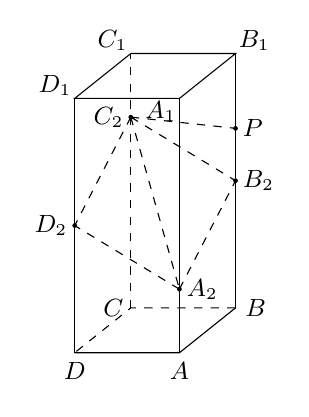
\begin{tikzpicture}[scale=0.95, font=\small]
  \coordinate (D)  at (0,0);
  \coordinate (A)  at (1.4,0);
  \coordinate (B)  at (2.15,0.6);
  \coordinate (C)  at (0.75,0.6);
  \coordinate (D1) at (0,3.4);
  \coordinate (A1) at (1.4,3.4);
  \coordinate (B1) at (2.15,4.0);
  \coordinate (C1) at (0.75,4.0);
  \coordinate (A2) at (1.4,0.85);
  \coordinate (B2) at (2.15,2.3);
  \coordinate (C2) at (0.75,3.15);
  \coordinate (D2) at (0,1.7);
  \coordinate (P)  at (2.15,3.0);
  \draw (D) -- (A) -- (B);
  \draw[dashed] (B) -- (C) -- (D);
  \draw (D) -- (D1)  (A) -- (A1)  (B) -- (B1);
  \draw[dashed] (C) -- (C1);
  \draw (D1) -- (A1) -- (B1) -- (C1) -- cycle;
  \draw[dashed] (C2) -- (A2)  (C2) -- (B2)  (C2) -- (D2)  (C2) -- (P);
  \draw[dashed] (A2) -- (B2)  (A2) -- (D2);
  \fill (A2) circle (0.9pt); \fill (B2) circle (0.9pt);
  \fill (C2) circle (0.9pt); \fill (D2) circle (0.9pt); \fill (P) circle (0.9pt);
  \node[below] at (D) {$D$};
  \node[below] at (A) {$A$};
  \node[right] at (B) {$B$};
  \node[left, inner sep=2.5pt] at (C) {$C$};
  \node[above left, inner sep=1pt] at (D1) {$D_1$};
  \node[below left, inner sep=1pt] at (A1) {$A_1$};
  \node[above right, inner sep=1pt] at (B1) {$B_1$};
  \node[above left, inner sep=1pt] at (C1) {$C_1$};
  \node[right, inner sep=2.5pt] at (A2) {$A_2$};
  \node[right, inner sep=2.5pt] at (B2) {$B_2$};
  \node[left, inner sep=2.5pt] at (C2) {$C_2$};
  \node[left, inner sep=2.5pt] at (D2) {$D_2$};
  \node[right, inner sep=2.5pt] at (P) {$P$};
\end{tikzpicture}
\end{center}
\nopagebreak[4]
  (1) 证明：$B_2C_2\parallel A_2D_2$；

  (2) 点 $P$ 在棱 $BB_1$ 上，当二面角 $P\text{-}A_2C_2\text{-}D_2$ 为 $150^\circ$ 时，求 $B_2P$。

\Needspace{4\baselineskip}
\textbf{解析}

  (1) 证明：$B_2C_2\parallel A_2D_2$；(2) 点 $P$ 在棱 $BB_1$ 上，二面角 $P\text{-}A_2C_2\text{-}D_2$ 为 $150^\circ$，求 $B_2P$。

\par\medskip

\textbf{建系（两问共用）}

\Needspace{5\baselineskip}
正四棱柱的底面是正方形、侧棱垂直底面，故可以 $A$ 为原点，$AB$、$AD$、$AA_1$ 为 $x,y,z$ 轴：
\nopagebreak[4]
\[A(0,0,0),\quad B(2,0,0),\quad C(2,2,0),\quad D(0,2,0)\]

\Needspace{5\baselineskip}
四个点分别沿各自侧棱上升给定高度：
\nopagebreak[4]
\[A_2(0,0,1),\quad B_2(2,0,2),\quad C_2(2,2,3),\quad D_2(0,2,2)\]

\par\medskip

\textbf{(1) 证明}

\Needspace{5\baselineskip}
直接计算两个向量：
\nopagebreak[4]
\[\overrightarrow{B_2C_2}=C_2-B_2=(2-2,\ 2-0,\ 3-2)=(0,\ 2,\ 1)\]
\nopagebreak[4]
\[\overrightarrow{A_2D_2}=D_2-A_2=(0-0,\ 2-0,\ 2-1)=(0,\ 2,\ 1)\]

\Needspace{5\baselineskip}
两个向量\textbf{完全相等}：
\nopagebreak[4]
\[\overrightarrow{B_2C_2}=\overrightarrow{A_2D_2}\]

故 $B_2C_2\parallel A_2D_2$（且 $\left|B_2C_2\right|=\left|A_2D_2\right|$，即 $A_2B_2C_2D_2$ 是平行四边形）。$\blacksquare$

\begin{gktip}
\textbf{书写提示}：由向量相等得出的是"平行且相等"，若严格按线线平行的定义作答，需补充说明 $B_2C_2$ 与 $A_2D_2$ \textbf{不共线}（由图易见它们在不同侧面上）。
\end{gktip}

\par\medskip

\textbf{(2) 解}

\Needspace{5\baselineskip}
设 $P$ 在棱 $BB_1$ 上，则
\nopagebreak[4]
\[P(2,\ 0,\ t),\qquad t\in[0,4]\]

\textbf{第一步，求两个半平面的法向量。}

\Needspace{5\baselineskip}
公共棱为 $A_2C_2$：
\nopagebreak[4]
\[\overrightarrow{A_2C_2}=C_2-A_2=(2,\ 2,\ 2)\]

\Needspace{5\baselineskip}
\textbf{平面 $PA_2C_2$}：
\nopagebreak[4]
\[\overrightarrow{A_2P}=P-A_2=(2,\ 0,\ t-1)\]

\nopagebreak[4]
\[\boldsymbol n_1=\overrightarrow{A_2C_2}\times\overrightarrow{A_2P}=\begin{vmatrix}\boldsymbol i&\boldsymbol j&\boldsymbol k\\ 2&2&2\\ 2&0&t-1\end{vmatrix}\]

\nopagebreak[4]
\[=\left(2(t-1)-0,\ \ 4-2(t-1),\ \ -4\right)=\left(2t-2,\ 6-2t,\ -4\right)\]

\Needspace{5\baselineskip}
\textbf{平面 $D_2A_2C_2$}：
\nopagebreak[4]
\[\overrightarrow{A_2D_2}=(0,\ 2,\ 1)\]

\nopagebreak[4]
\[\boldsymbol n_2=\overrightarrow{A_2C_2}\times\overrightarrow{A_2D_2}=\begin{vmatrix}\boldsymbol i&\boldsymbol j&\boldsymbol k\\ 2&2&2\\ 0&2&1\end{vmatrix}=(2-4,\ \ 0-2,\ \ 4-0)=(-2,\ -2,\ 4)\]

\nopagebreak[4]
\[\left|\boldsymbol n_2\right|=\sqrt{4+4+16}=\sqrt{24}=2\sqrt6\]

\Needspace{5\baselineskip}
\textbf{第二步，计算点积（注意它与 $t$ 无关）。}
\nopagebreak[4]
\[\boldsymbol n_1\cdot\boldsymbol n_2=(2t-2)(-2)+(6-2t)(-2)+(-4)(4)\]
\nopagebreak[4]
\[=-4t+4-12+4t-16=-24\]

\textbf{含 $t$ 的项恰好抵消}，这是本题的一个便利之处。

\textbf{第三步，用二面角条件建立方程。}

\Needspace{5\baselineskip}
二面角为 $150^\circ$，$\left|\cos150^\circ\right|=\dfrac{\sqrt3}2$：
\nopagebreak[4]
\[\frac{\left|\boldsymbol n_1\cdot\boldsymbol n_2\right|}{\left|\boldsymbol n_1\right|\left|\boldsymbol n_2\right|}=\frac{24}{\left|\boldsymbol n_1\right|\times2\sqrt6}=\frac{\sqrt3}2\]

\nopagebreak[4]
\[\left|\boldsymbol n_1\right|=\frac{24\times2}{2\sqrt6\times\sqrt3}=\frac{48}{2\sqrt{18}}=\frac{48}{6\sqrt2}=\frac{8}{\sqrt2}=4\sqrt2\]

\Needspace{5\baselineskip}
\textbf{第四步，解出 $t$。}
\nopagebreak[4]
\[\left|\boldsymbol n_1\right|^{2}=(2t-2)^{2}+(6-2t)^{2}+16=32\]

\nopagebreak[4]
\[\left(4t^{2}-8t+4\right)+\left(4t^{2}-24t+36\right)+16=32\]
\nopagebreak[4]
\[8t^{2}-32t+56=32\ \Longrightarrow\ 8t^{2}-32t+24=0\ \Longrightarrow\ t^{2}-4t+3=0\]

\nopagebreak[4]
\[(t-1)(t-3)=0\ \Longrightarrow\ t=1\ \text{\text{或}}\ t=3\]

（两个值都在 $[0,4]$ 内，均合法。）

\textbf{第五步，求 $B_2P$。}

\Needspace{5\baselineskip}
$B_2(2,0,2)$ 与 $P(2,0,t)$ 只有竖坐标不同：
\nopagebreak[4]
\[B_2P=|t-2|\]

\begin{itemize}
\item $t=1$ 时：$B_2P=1$
\item $t=3$ 时：$B_2P=1$
\end{itemize}

\textbf{两种情形给出相同结果}（$P$ 在 $B_2$ 上方或下方各 $1$ 个单位，由对称性可预见）。

\textbf{所以 $B_2P=1$。}

\begin{gktip}
\textbf{方法总结}：二面角问题的通法是"两个半平面各求一个法向量，再用夹角公式"。本题的加速点有二：① $\boldsymbol n_1\cdot\boldsymbol n_2$ 中 $t$ 自动抵消，使方程只剩 $\left|\boldsymbol n_1\right|$ 一个未知量；② 二次方程的两个根给出对称的两点，答案唯一。\textbf{注意二面角是钝角（$150^\circ$）时，法向量夹角的余弦要取绝对值再判断。}
\end{gktip}

\gkanswer{答案（1）：见解析版}

\gkanswer{答案（2）：$B_2P=1$}

\par\medskip

\end{answer}
\begin{answer}
\gksolhead{19}{12 分}

\textbf{题目}（12 分）：

已知函数 $f(x)=a\left(\mathrm e^{x}+a\right)-x$。

  (1) 讨论 $f(x)$ 的单调性；

  (2) 证明：当 $a>0$ 时，$f(x)>2\ln a+\dfrac32$。

\Needspace{4\baselineskip}
\textbf{解析}

\par\medskip

\textbf{(1) 解}

\Needspace{5\baselineskip}
先展开：
\nopagebreak[4]
\[f(x)=a\mathrm e^{x}+a^{2}-x\]

\Needspace{5\baselineskip}
（注意 $a^{2}$ 是常数，求导时消失。）

\nopagebreak[4]
\[f'(x)=a\mathrm e^{x}-1\]

\textbf{分类讨论 $a$ 的符号：}

\textbf{情形一：$a\le0$。}

\Needspace{5\baselineskip}
此时 $a\mathrm e^{x}\le0$（因 $\mathrm e^{x}>0$），故
\nopagebreak[4]
\[f'(x)=a\mathrm e^{x}-1\le-1<0\]

$f(x)$ 在 $\mathbf R$ 上\textbf{单调递减}。

\textbf{情形二：$a>0$。}

\Needspace{5\baselineskip}
令 $f'(x)=0$：
\nopagebreak[4]
\[a\mathrm e^{x}=1\ \Longrightarrow\ \mathrm e^{x}=\frac1a\ \Longrightarrow\ x=-\ln a\]

因 $a\mathrm e^{x}$ 关于 $x$ 单调递增：
\begin{itemize}
\item 当 $x<-\ln a$ 时 $f'(x)<0$，$f$ 递减；
\item 当 $x>-\ln a$ 时 $f'(x)>0$，$f$ 递增。
\end{itemize}

\textbf{综上}：
\begin{itemize}
\item $a\le0$ 时，$f(x)$ 在 $\mathbf R$ 上单调递减；
\item $a>0$ 时，$f(x)$ 在 $(-\infty,-\ln a)$ 上单调递减，在 $(-\ln a,+\infty)$ 上单调递增。
\end{itemize}

\par\medskip

\textbf{(2) 证明}

\textbf{第一步，求最小值。}

\Needspace{5\baselineskip}
由 (1)，$a>0$ 时 $f$ 在 $x=-\ln a$ 处取得\textbf{最小值}：
\nopagebreak[4]
\[f(-\ln a)=a\mathrm e^{-\ln a}+a^{2}-(-\ln a)=a\cdot\frac1a+a^{2}+\ln a=a^{2}+\ln a+1\]

（这里用了 $\mathrm e^{-\ln a}=\dfrac1a$。）

\textbf{第二步，转化为关于 $a$ 的不等式。}

\Needspace{5\baselineskip}
只需证明最小值大于右端：
\nopagebreak[4]
\[a^{2}+\ln a+1>2\ln a+\frac32\]

\Needspace{5\baselineskip}
移项整理：
\nopagebreak[4]
\[a^{2}-\ln a-\frac12>0\qquad(a>0)\]

\textbf{第三步，构造函数求其最小值。}

\Needspace{5\baselineskip}
令
\nopagebreak[4]
\[g(a)=a^{2}-\ln a-\frac12,\qquad a>0\]

\nopagebreak[4]
\[g'(a)=2a-\frac1a=\frac{2a^{2}-1}a\]

\Needspace{5\baselineskip}
令 $g'(a)=0$：
\nopagebreak[4]
\[a^{2}=\frac12\ \Longrightarrow\ a=\frac1{\sqrt2}\quad(a>0)\]

\begin{itemize}
\item $0<a<\dfrac1{\sqrt2}$ 时 $g'(a)<0$，递减；
\item $a>\dfrac1{\sqrt2}$ 时 $g'(a)>0$，递增。
\end{itemize}

\Needspace{5\baselineskip}
故 $g$ 在 $a=\dfrac1{\sqrt2}$ 处取最小值：
\nopagebreak[4]
\[g\left(\frac1{\sqrt2}\right)=\frac12-\ln\frac1{\sqrt2}-\frac12=-\ln\frac1{\sqrt2}=\ln\sqrt2=\frac12\ln2\]

\textbf{第四步，下结论。}

\Needspace{5\baselineskip}
因 $\ln2\approx0.693>0$：
\nopagebreak[4]
\[g(a)\ge\frac12\ln2>0\qquad\text{\text{对一切} }a>0\]

\Needspace{5\baselineskip}
因此
\nopagebreak[4]
\[f(x)\ge f(-\ln a)=a^{2}+\ln a+1>2\ln a+\frac32\qquad\blacksquare\]

\begin{gktip}
\textbf{方法总结}：这是「双变量不等式」的标准处理路线——
1. 对 $x$ 求最小值，把含 $x$ 的问题变成只含参数 $a$ 的问题（\textbf{消元}）；
2. 对得到的 $a$ 的不等式再构造函数、再求最值（\textbf{二次求导}）。

关键是第一步要意识到"证 $f(x)>$ 某式"等价于"证 $f_{\min}>$ 某式"。另外注意最后是\textbf{严格大于}：$g$ 的最小值 $\dfrac12\ln2$ 严格为正，所以结论中的严格不等号成立。
\end{gktip}

\gkanswer{答案（1）：$f'(x)=a\mathrm e^x-1$。$a\le0$：$a\mathrm e^x\le0$，故 $f'(x)<0$，$f$ 在 $\mathbf R$ 上单调递减；$a>0$：由 $f'(x)=0$ 得 $x=-\ln a$，$f$ 在 $(-\infty,-\ln a)$ 递减、在 $(-\ln a,+\infty)$ 递增。}

\gkanswer{答案（2）：见解析版}

\par\medskip

\end{answer}
\begin{answer}
\gksolhead{20}{12 分}

\textbf{题目}（12 分）：

设等差数列 $\left\{a_n\right\}$ 的公差为 $d$，且 $d>1$。令 $b_n=\dfrac{n^{2}+n}{a_n}$，记 $S_n$，$T_n$ 分别为数列 $\left\{a_n\right\}$，$\left\{b_n\right\}$ 的前 $n$ 项和。

  (1) 若 $3a_2=3a_1+a_3$，$S_3+T_3=21$，求 $\left\{a_n\right\}$ 的通项公式；

  (2) 若 $\left\{b_n\right\}$ 为等差数列，且 $S_{99}-T_{99}=99$，求 $d$。

\Needspace{4\baselineskip}
\textbf{解析}

\par\medskip

\textbf{(1) 解}

\Needspace{5\baselineskip}
\textbf{第一步，由 $3a_2=3a_1+a_3$ 找到 $a_1$ 与 $d$ 的关系。}
\nopagebreak[4]
\[3\left(a_1+d\right)=3a_1+\left(a_1+2d\right)\]
\nopagebreak[4]
\[3a_1+3d=4a_1+2d\ \Longrightarrow\ a_1=d\]

\Needspace{5\baselineskip}
于是
\nopagebreak[4]
\[a_n=a_1+(n-1)d=d+(n-1)d=nd\]

\Needspace{5\baselineskip}
\textbf{第二步，求 $b_n$。}
\nopagebreak[4]
\[b_n=\frac{n^{2}+n}{a_n}=\frac{n(n+1)}{nd}=\frac{n+1}d\]

\Needspace{5\baselineskip}
\textbf{第三步，计算 $S_3$ 与 $T_3$。}
\nopagebreak[4]
\[S_3=a_1+a_2+a_3=d+2d+3d=6d\]
\nopagebreak[4]
\[T_3=b_1+b_2+b_3=\frac2d+\frac3d+\frac4d=\frac9d\]

\Needspace{5\baselineskip}
\textbf{第四步，解方程。}
\nopagebreak[4]
\[6d+\frac9d=21\]

\Needspace{5\baselineskip}
两边乘 $d$（$d>1>0$）：
\nopagebreak[4]
\[6d^{2}-21d+9=0\ \Longrightarrow\ 2d^{2}-7d+3=0\]

\nopagebreak[4]
\[d=\frac{7\pm\sqrt{49-24}}4=\frac{7\pm5}4\]

\Needspace{5\baselineskip}
得 $d=3$ 或 $d=\dfrac12$。由 $d>1$ 舍去 $\dfrac12$：
\nopagebreak[4]
\[d=3\]

\textbf{所以 $a_n=3n$。}

\par\medskip

\textbf{(2) 解}

\Needspace{5\baselineskip}
\textbf{第一步（本题关键）：$\left\{b_n\right\}$ 为等差数列意味着什么？}

\nopagebreak[4]
\[b_n=\frac{n(n+1)}{a_n}=\frac{n(n+1)}{dn+\left(a_1-d\right)}\]

分子是 $n$ 的\textbf{二次式}，分母是\textbf{一次式}。要使商为 $n$ 的一次式（等差数列的通项必是一次式），必须\textbf{分母整除分子}。

\Needspace{5\baselineskip}
分母 $dn+\left(a_1-d\right)$ 的零点为
\nopagebreak[4]
\[n=\frac{d-a_1}d\]

\Needspace{5\baselineskip}
要整除 $n(n+1)$，这个零点必须是分子的零点，即
\nopagebreak[4]
\[\frac{d-a_1}d=0\qquad\text{\text{或}}\qquad\frac{d-a_1}d=-1\]

\textbf{情形一：$a_1=d$}

此时 $a_n=nd$，$b_n=\dfrac{n(n+1)}{nd}=\dfrac{n+1}d$（首项 $\dfrac2d$、公差 $\dfrac1d$ 的等差数列）

\textbf{情形二：$a_1=2d$}

（由 $\dfrac{d-a_1}d=-1$ 得 $d-a_1=-d$。）
此时 $a_n=2d+(n-1)d=(n+1)d$，$b_n=\dfrac{n(n+1)}{(n+1)d}=\dfrac nd$（首项 $\dfrac1d$、公差 $\dfrac1d$）

\textbf{第二步，分别代入 $S_{99}-T_{99}=99$。}

预备：$\displaystyle\sum_{n=1}^{99}n=\frac{99\times100}2=4950$。

\par\medskip

\Needspace{5\baselineskip}
\textbf{情形一（$a_n=nd$，$b_n=\dfrac{n+1}d$）：}
\nopagebreak[4]
\[S_{99}=d\sum_{n=1}^{99}n=4950d\]
\nopagebreak[4]
\[T_{99}=\frac1d\sum_{n=1}^{99}(n+1)=\frac1d\left(4950+99\right)=\frac{5049}d\]

\nopagebreak[4]
\[4950d-\frac{5049}d=99\]

\Needspace{5\baselineskip}
两边乘 $d$ 并整理：
\nopagebreak[4]
\[4950d^{2}-99d-5049=0\]

\Needspace{5\baselineskip}
同除以 $99$：
\nopagebreak[4]
\[50d^{2}-d-51=0\]

\nopagebreak[4]
\[d=\frac{1\pm\sqrt{1+4\times50\times51}}{100}=\frac{1\pm\sqrt{10201}}{100}=\frac{1\pm101}{100}\]

得 $d=\dfrac{102}{100}=\dfrac{51}{50}$ 或 $d=-1$。

由 $d>1$：$\dfrac{51}{50}=1.02>1$  \textbf{符合}。

\par\medskip

\Needspace{5\baselineskip}
\textbf{情形二（$a_n=(n+1)d$，$b_n=\dfrac nd$）：}
\nopagebreak[4]
\[S_{99}=d\sum_{n=1}^{99}(n+1)=d\left(4950+99\right)=5049d\]
\nopagebreak[4]
\[T_{99}=\frac1d\sum_{n=1}^{99}n=\frac{4950}d\]

\nopagebreak[4]
\[5049d-\frac{4950}d=99\ \Longrightarrow\ 5049d^{2}-99d-4950=0\]

\Needspace{5\baselineskip}
同除以 $99$：
\nopagebreak[4]
\[51d^{2}-d-50=0\ \Longrightarrow\ (51d+50)(d-1)=0\]

得 $d=1$ 或 $d=-\dfrac{50}{51}$。

\textbf{两者都不满足 $d>1$}（注意 $d>1$ 是\textbf{严格}大于），情形二\textbf{舍去}。

\textbf{所以 $d=\dfrac{51}{50}$。}

\begin{gktip}
\textbf{方法总结}：本题第 (2) 问的难点在于把"$\left\{b_n\right\}$ 是等差数列"这个抽象条件\textbf{翻译成整除条件}。核心洞察是：等差数列的通项必是 $n$ 的一次式，而 $b_n$ 是"二次 ÷ 一次"，故只有分母整除分子时商才能是一次式。这一步想通，剩下的就是两次常规计算。

另外注意题目给的 $d>1$ 不是摆设——它恰好淘汰掉情形二的 $d=1$，保证答案唯一。
\end{gktip}

\gkanswer{答案（1）：$a_n=3n$}

\gkanswer{答案（2）：$d=\dfrac{51}{50}$}

\par\medskip

\end{answer}
\begin{answer}
\gksolhead{21}{12 分}

\textbf{题目}（12 分）：

甲、乙两人投篮，每次由其中一人投篮，规则如下：若命中则此人继续投篮，若未命中则换为对方投篮。无论之前投篮情况如何，甲每次投篮的命中率均为 $0.6$，乙每次投篮的命中率均为 $0.8$。由抽签决定第 $1$ 次投篮的人选，第 $1$ 次投篮的人是甲、乙的概率各为 $0.5$。

  (1) 求第 $2$ 次投篮的人是乙的概率；

  (2) 求第 $i$ 次投篮的人是甲的概率；

  (3) 已知：若随机变量 $X_i$ 服从两点分布，且 $P\left(X_i=1\right)=1-P\left(X_i=0\right)=q_i$，$i=1,2,\cdots,n$，则 $E\left(\displaystyle\sum_{i=1}^{n}X_i\right)=\displaystyle\sum_{i=1}^{n}q_i$。记前 $n$ 次（即从第 $1$ 次到第 $n$ 次投篮）中甲投篮的次数为 $Y$，求 $E(Y)$。

\Needspace{4\baselineskip}
\textbf{解析}

\par\medskip

\textbf{(1) 解}

第 2 次投篮的人是乙，有两条互斥路径：

\Needspace{5\baselineskip}
\textbf{路径一}：第 1 次是甲投（概率 $0.5$），且甲\textbf{未命中}（概率 $1-0.6=0.4$），于是换乙：
\nopagebreak[4]
\[0.5\times0.4=0.2\]

\Needspace{5\baselineskip}
\textbf{路径二}：第 1 次是乙投（概率 $0.5$），且乙\textbf{命中}（概率 $0.8$），于是乙继续：
\nopagebreak[4]
\[0.5\times0.8=0.4\]

\Needspace{5\baselineskip}
由互斥事件的加法：
\nopagebreak[4]
\[P=0.2+0.4=0.6\]

\textbf{所以第 2 次投篮的人是乙的概率为 $0.6$。}

\par\medskip

\textbf{(2) 解}

设 $p_i$ 表示"第 $i$ 次投篮的人是甲"的概率，则 $p_1=0.5$。

\textbf{建立递推关系。} 第 $i+1$ 次是甲投篮，同样有两条路径：

\begin{itemize}
\item 第 $i$ 次是甲（概率 $p_i$）且\textbf{命中}（$0.6$）→ 甲继续；
\item 第 $i$ 次是乙（概率 $1-p_i$）且\textbf{未命中}（$1-0.8=0.2$）→ 换甲。
\end{itemize}

\nopagebreak[4]
\[p_{i+1}=0.6p_i+0.2\left(1-p_i\right)=0.4p_i+0.2\]

\Needspace{5\baselineskip}
\textbf{用不动点法求通项。} 令 $p=0.4p+0.2$，解得不动点
\nopagebreak[4]
\[p=\frac{0.2}{0.6}=\frac13\]

\Needspace{5\baselineskip}
两边减去 $\dfrac13$：
\nopagebreak[4]
\[p_{i+1}-\frac13=0.4\left(p_i-\frac13\right)\]

\Needspace{5\baselineskip}
故 $\left\{p_i-\dfrac13\right\}$ 是公比 $0.4=\dfrac25$ 的等比数列，首项
\nopagebreak[4]
\[p_1-\frac13=\frac12-\frac13=\frac16\]

\nopagebreak[4]
\[p_i-\frac13=\frac16\left(\frac25\right)^{i-1}\]

\Needspace{5\baselineskip}
\textbf{所以}
\nopagebreak[4]
\[p_i=\frac13+\frac16\left(\frac25\right)^{i-1}\]

\textbf{检验}：$i=1$ 时 $p_1=\dfrac13+\dfrac16=\dfrac12$ ；$i=2$ 时 $p_2=\dfrac13+\dfrac16\times\dfrac25=\dfrac13+\dfrac1{15}=\dfrac25=0.4$，与 (1) 的答案互补（$1-0.6=0.4$）

\par\medskip

\textbf{(3) 解}

\Needspace{5\baselineskip}
设 $X_i=\begin{cases}1,&\text{\text{第} }i\text{ \text{次是甲投篮}}\\ 0,&\text{\text{否则}}\end{cases}$，则 $X_i$ 服从两点分布，$P\left(X_i=1\right)=p_i$，且
\nopagebreak[4]
\[Y=\sum_{i=1}^{n}X_i\]

\Needspace{5\baselineskip}
由题目给出的结论（期望的可加性）：
\nopagebreak[4]
\[E(Y)=\sum_{i=1}^{n}p_i=\sum_{i=1}^{n}\left[\frac13+\frac16\left(\frac25\right)^{i-1}\right]\]

\textbf{拆成两部分求和：}

\Needspace{5\baselineskip}
\textbf{常数部分}：
\nopagebreak[4]
\[\sum_{i=1}^{n}\frac13=\frac n3\]

\Needspace{5\baselineskip}
\textbf{等比部分}（首项 $\dfrac16$、公比 $\dfrac25$、共 $n$ 项）：
\nopagebreak[4]
\[\sum_{i=1}^{n}\frac16\left(\frac25\right)^{i-1}=\frac16\cdot\frac{1-\left(\dfrac25\right)^{n}}{1-\dfrac25}=\frac16\cdot\frac53\left[1-\left(\frac25\right)^{n}\right]=\frac5{18}\left[1-\left(\frac25\right)^{n}\right]\]

\Needspace{5\baselineskip}
\textbf{所以}
\nopagebreak[4]
\[E(Y)=\frac5{18}\left[1-\left(\frac25\right)^{n}\right]+\frac n3\]

\begin{gktip}
\textbf{方法总结}：这是一道典型的\textbf{马尔可夫链}问题（虽然中学不用这个名词）。三问层层递进：
1. 第 (1) 问用\textbf{全概率公式}枚举路径；
2. 第 (2) 问把路径分析\textbf{一般化为递推式}，再用不动点法（形如 $p_{n+1}=Ap_n+B$ 的递推，永远先解 $p=Ap+B$ 找不动点，再化为等比数列）；
3. 第 (3) 问用题目\textbf{恩赐的期望可加性}，把求 $Y$ 的分布这一难事化为求 $p_i$ 的和。

值得注意的是 $p_i\to\dfrac13$（$i\to\infty$），意味着长期来看甲投篮的比例趋于 $\dfrac13$——这符合直觉：乙的命中率更高，一旦拿到球会持续更久。
\end{gktip}

\gkanswer{答案（1）：$0.6$}

\gkanswer{答案（2）：$p_i=\dfrac13+\dfrac16\left(\dfrac25\right)^{i-1}$}

\gkanswer{答案（3）：$E(Y)=\dfrac5{18}\left[1-\left(\dfrac25\right)^n\right]+\dfrac n3$}

\par\medskip

\end{answer}
\begin{answer}
\gksolhead{22}{12 分}

\textbf{题目}（12 分）：

在直角坐标系 $xOy$ 中，点 $P$ 到 $x$ 轴的距离等于点 $P$ 到点 $\left(0,\dfrac12\right)$ 的距离，记动点 $P$ 的轨迹为 $W$。

  (1) 求 $W$ 的方程；

  (2) 已知矩形 $ABCD$ 有三个顶点在 $W$ 上，证明：矩形 $ABCD$ 的周长大于 $3\sqrt3$。

\par\medskip

\Needspace{4\baselineskip}
\textbf{解析}

\par\medskip

\textbf{(1) 解}

设 $P(x,y)$。

\begin{itemize}
\item $P$ 到 $x$ 轴的距离：$|y|$
\item $P$ 到点 $\left(0,\dfrac12\right)$ 的距离：$\sqrt{x^{2}+\left(y-\dfrac12\right)^{2}}$
\end{itemize}

\Needspace{5\baselineskip}
由题意：
\nopagebreak[4]
\[|y|=\sqrt{x^{2}+\left(y-\frac12\right)^{2}}\]

\Needspace{5\baselineskip}
两边平方：
\nopagebreak[4]
\[y^{2}=x^{2}+y^{2}-y+\frac14\]

\Needspace{5\baselineskip}
化简（$y^{2}$ 抵消）：
\nopagebreak[4]
\[0=x^{2}-y+\frac14\ \Longrightarrow\ y=x^{2}+\frac14\]

\textbf{所以 $W$ 的方程为 $y=x^{2}+\dfrac14$。}

\begin{gktip}
顺带一提：这条抛物线的焦点恰是 $\left(0,\dfrac12\right)$、准线恰是 $x$ 轴，题目描述的正是抛物线的定义。
\end{gktip}

\par\medskip

\textbf{(2) 证明}

\textbf{第一步，设参并利用抛物线的斜率特性。}

\Needspace{5\baselineskip}
设矩形的三个顶点在 $W$ 上，且\textbf{直角顶点为 $B$}（三个顶点中必有一个是与另两个都相邻的，即直角顶点）。记
\nopagebreak[4]
\[A\left(a,\ a^{2}+\frac14\right),\quad B\left(b,\ b^{2}+\frac14\right),\quad C\left(c,\ c^{2}+\frac14\right)\]

\Needspace{5\baselineskip}
\textbf{关键性质}：抛物线 $y=x^{2}+\dfrac14$ 上两点连线的斜率等于两横坐标之和：
\nopagebreak[4]
\[k_{AB}=\frac{\left(a^{2}+\frac14\right)-\left(b^{2}+\frac14\right)}{a-b}=\frac{a^{2}-b^{2}}{a-b}=a+b\]

\Needspace{5\baselineskip}
同理 $k_{BC}=b+c$。记
\nopagebreak[4]
\[m=a+b,\qquad n=b+c\]

\Needspace{5\baselineskip}
由 $AB\perp BC$：
\nopagebreak[4]
\[mn=-1\qquad(\ast)\]

\Needspace{5\baselineskip}
\textbf{第二步，用 $m$、$n$ 表示两条边长。}

\nopagebreak[4]
\[|AB|=|a-b|\sqrt{1+k_{AB}^{2}}=|a-b|\sqrt{1+m^{2}}\]
\nopagebreak[4]
\[|BC|=|b-c|\sqrt{1+n^{2}}\]

\Needspace{5\baselineskip}
引入 $u=2b$，则由 $a=m-b$、$c=n-b$：
\nopagebreak[4]
\[a-b=m-2b=m-u,\qquad b-c=2b-n=u-n\]

\Needspace{5\baselineskip}
于是\textbf{半周长}为
\nopagebreak[4]
\[L=|AB|+|BC|=|m-u|\sqrt{1+m^{2}}+|u-n|\sqrt{1+n^{2}}\]

\textbf{第三步，对 $u$ 求下确界。}

\Needspace{5\baselineskip}
$L$ 是 $u$ 的\textbf{分段线性函数}，其折点在 $u=n$ 与 $u=m$。由 $(\ast)$ 知 $m$、$n$ 异号，不妨设
\nopagebreak[4]
\[m>0>n,\qquad n=-\frac1m\]

\begin{itemize}
\item 当 $u<n$ 或 $u>m$ 时，两项同时增大，$L$ 更大；
\item 当 $n\le u\le m$ 时，$L$ 线性，最小值在端点 $u=m$ 或 $u=n$ 取得：
\end{itemize}

\nopagebreak[4]
\[L(m)=(m-n)\sqrt{1+n^{2}},\qquad L(n)=(m-n)\sqrt{1+m^{2}}\]

\Needspace{5\baselineskip}
故
\nopagebreak[4]
\[L>\left(m-n\right)\min\left\{\sqrt{1+m^{2}},\ \sqrt{1+n^{2}}\right\}\]

\textbf{为何是严格不等号}：在 $u=m$ 处 $a=b$（$A$ 与 $B$ 重合），在 $u=n$ 处 $b=c$（$B$ 与 $C$ 重合），都使矩形退化，\textbf{实际取不到}，故 $L$ 严格大于该下确界。

\textbf{第四步，对 $m$ 求最小值。}

\Needspace{5\baselineskip}
不妨设 $m\ge1$（若 $m<1$ 则 $|n|=\dfrac1m>1$，把 $m$、$n$ 的角色对调即可，由对称性不影响结论）。此时 $|n|=\dfrac1m\le m$，故 $\sqrt{1+n^{2}}$ 较小：
\nopagebreak[4]
\[L>\left(m+\frac1m\right)\sqrt{1+\frac1{m^{2}}}=\frac{m^{2}+1}m\cdot\frac{\sqrt{m^{2}+1}}m=\frac{\left(m^{2}+1\right)^{3/2}}{m^{2}}\]

\Needspace{5\baselineskip}
令 $v=m^{2}\ge1$，定义
\nopagebreak[4]
\[g(v)=\frac{(v+1)^{3/2}}v\]

\Needspace{5\baselineskip}
求导：
\nopagebreak[4]
\[g'(v)=\frac{\dfrac32(v+1)^{1/2}\cdot v-(v+1)^{3/2}}{v^{2}}=\frac{(v+1)^{1/2}\left[\dfrac32v-(v+1)\right]}{v^{2}}=\frac{(v+1)^{1/2}\left(\dfrac v2-1\right)}{v^{2}}\]

\Needspace{5\baselineskip}
令 $g'(v)=0$ 得 $v=2$；且 $v<2$ 时 $g'<0$、$v>2$ 时 $g'>0$，故 $v=2$ 是\textbf{最小值点}：
\nopagebreak[4]
\[g(2)=\frac{3^{3/2}}2=\frac{3\sqrt3}2\]

\Needspace{5\baselineskip}
\textbf{第五步，得出结论。}

\nopagebreak[4]
\[L>\frac{3\sqrt3}2\ \Longrightarrow\ \text{\text{周长}}=2L>3\sqrt3\qquad\blacksquare\]

\begin{gktip}
\textbf{方法总结}：本题是全卷最难的一题，破题链条为：
1. \textbf{抛物线的斜率特性}（两点连线斜率 $=$ 横坐标之和）把几何条件 $AB\perp BC$ 转化为简洁的 $mn=-1$——这是关键第一步；
2. 引入 $u=2b$ 后，半周长成为 $u$ 的\textbf{分段线性函数}，其最小值必在折点，从而消去一个变量；
3. 剩下的单变量最值用换元 $v=m^{2}$ 加求导解决。

\textbf{考试策略}：这类题的第 (1) 问（求轨迹方程）是纯送分的，一定要拿下；第 (2) 问属于压轴中的压轴，及格线至 120 分段的学生应果断跳过。
\end{gktip}

\gkanswer{答案（1）：$y=x^2+\dfrac14$}

\gkanswer{答案（2）：见解析版}

\end{answer}